\documentclass[usenames,dvipsnames,notes,11pt,aspectratio=169,hyperref={colorlinks=true, linkcolor=blue}]{beamer}
\usepackage{ifthen}
\usepackage[T1]{fontenc}
\usepackage{xcolor}
\usepackage{pgfplots}
\usepackage{amsmath}
\usepackage{centernot}
\usepackage{pifont}
\usepackage{tabularx}
\usepackage{makecell}
\usepackage{cuted}
\usepackage{booktabs}
\usepackage{array}
\usepackage{textcomp}
\usepackage{setspace}
\usepackage{xspace}
\usepackage{subcaption}
\usepackage{tikz}
\usepackage{pdfcomment}
%\newcommand{\pdfnote}[1]{\marginnote{\pdfcomment[icon=note]{#1}}}
\newcommand{\pdfnote}[1]{}

\usepackage{pgfpages}
%\setbeameroption{show notes on second screen}


\input ../beamer-style
\input ../std-macros
\input ../macros

\newcommand{\pt}{\partial}

\AtBeginSection[]
{
    \begin{frame}
        \frametitle{Table of Contents}
        \tableofcontents[currentsection]
    \end{frame}
}
\parskip=10pt

\title[DS-GA-1011]{Neural Sequence Generation}
\author[He He]{He He
}
\institute[NYU]{
    \includegraphics[height=1cm]{../figures/nyu-logo}\\
}
\date{September 25, 2023}

\begin{document}
\begin{frame}
\titlepage
\end{frame}

% TODO: add sections

\begin{frame}
    {Review: sequence representation}
    \begin{wideitemize}
        \item {\bf Encoders} represent a sequence of tokens as a sequence of embeddings
        \item Each embedding is a {\bf contextualized representation} of the token
        \item We can then use the embeddings for classification or sequence labeling
        \item What if we want to predict a sequence of tokens from the input sequence (e.g., machine translation)?
    \end{wideitemize}
\end{frame}

\begin{frame}
    {Sequence generation}
    \begin{wideitemize}[<+->]
        \item Sequence classification: $h: \sV^n \rightarrow \red{\pc{0,\ldots,K}}$
            \begin{itemize}[<.->]
                \item Sentiment classification
                \item Next word prediction
            \end{itemize}
        \item Sequence labeling: $h: \sV^n \rightarrow \red{\pc{0,\ldots,K}^n}$
            \begin{itemize}[<.->]
                \item Part-of-speech tagging 
                \item Name entity recognition 
            \end{itemize}

        \item Sequence generation: $h: \sV_{\text{in}}^n \rightarrow \red{\sV_{\text{out}}^m}$
            \begin{itemize}[<.->]
                \item Summarization: document to summary
                \item Open-domain dialogue: context to response
                \item Parsing: sentence to linearized trees
                \item In general: \blue{sequence to sequence}
            \end{itemize}
    \end{wideitemize}
   
    \pause{
        Main difference (and challenge) is that the \red{output space} is much larger.}
\end{frame}

\begin{frame}
    {Reduce generation to classification}
    Setup:\\
    \begin{itemize}
        \item Input: $x \in \sV_{\text{in}}^n$, e.g. \textit{Le Programme    a    ate    mis    en application}
        \item Output: $y \in \sV_{\text{out}}^m$, e.g., \textit{The program has been implemented }
    \end{itemize}
    \pause

    Consider a probabilistic model $p(y\mid x)$\\
    \begin{itemize}[<+->]
        \item Can we reduce it to classification?
        \item Decompose the problem using \textbf{chain rule of probability} 
            \begin{align*}
                p(y\mid x) &= p(y_1\mid x)p(y_2\mid y_1, x)\ldots p(y_m\mid y_{m-1},\ldots,y_1, x) \\
                &= \prod_{i=1}^m p(y_i\mid y_{<i}, x)
            \end{align*}
        \item We only need to model the \blue{next word distribution} $p(y_i\mid y_{<i}, x)$ now.
    \end{itemize}
\end{frame}

\begin{frame}
    {Reduce generation to classification}
    We want to model the {next word distribution} $p(\red{y_i}\mid \blue{y_{<i}}, \green{x})$.\\
    \begin{itemize}
        \item Input: a sequence of tokens (\blue{prefix} and \green{input})
        \item Output: the \red{next word} from the output vocabulary
        %\item We have reduced it to a classification problem.
    \end{itemize}

    \pause
    Reduce generation to a sequence of classification problems:\\
    \begin{enumerate}[<+->]
        \item \green{Le Programme    a    ate    mis    en application}
            $\to$ \red{The}
        \item \green{Le Programme    a    ate    mis    en application},
            \blue{The}
            $\to$ \red{program}
        \item \green{Le Programme    a    ate    mis    en application},
            \blue{The program}
            $\to$ \red{has}
        \item \green{Le Programme    a    ate    mis    en application},
            \blue{The program has}
            $\to$ \red{been}
        \item ...
    \end{enumerate}

    \pause
    We know how to solve each sequence classification problem! 

    %\pause
    %We can use an RNN to model $p(y_i\mid {y_{<i}}, {x})$.
    %\begin{figure}
    %    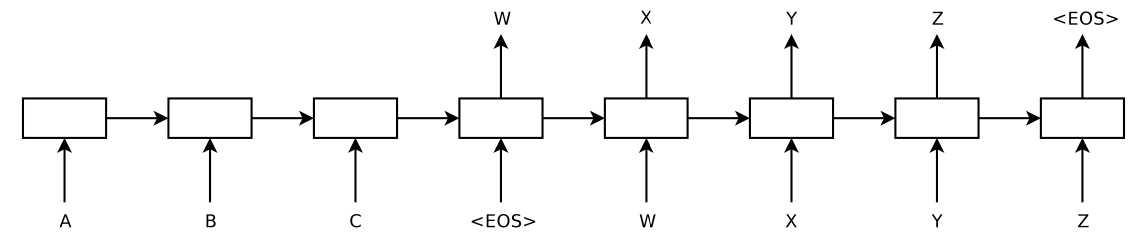
\includegraphics[height=2.5cm]{figures/s2s-ilya}
    %    \caption{From \href{https://arxiv.org/abs/1409.3215}{Sequence to Sequence Learning with Neural Networks} [Sutskever et al., 2014]}
    %\end{figure}
\end{frame}

\begin{frame}
    {The encoder-decoder architecture}

    Model the {input} (e.g., French) and the {output} (e.g., English) {\it separately}.\\
    \begin{figure}
        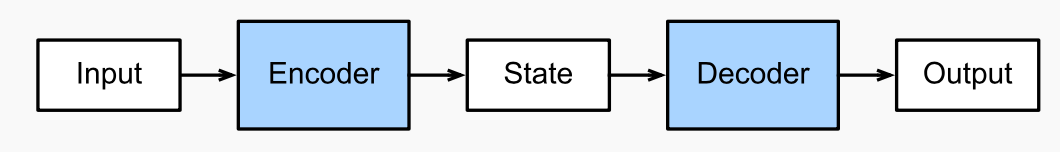
\includegraphics[height=1.5cm]{figures/enc-dec}
        \caption{10.6.1 from \href{https://d2l.ai/chapter_recurrent-modern/encoder-decoder.html}{d2l.ai}}
    \end{figure}

    \pause
    \begin{itemize}
        \item The \textbf{encoder} reads the input:
            $$
            \mathrm{Encoder}(x_1,\ldots,x_n) = \pb{h_1,\ldots,h_n}$$ where $h_i\in\BR^d$ are hidden states / embeddings.
        \pause
        \item The \textbf{decoder}  writes the output:
            $$\mathrm{Decoder}(h_1,\ldots,h_n) = \pb{y_1,\ldots, y_m}$$.
    \end{itemize}
\end{frame}

\begin{frame}
    {RNN encoder-decoder model}
    \begin{figure}
        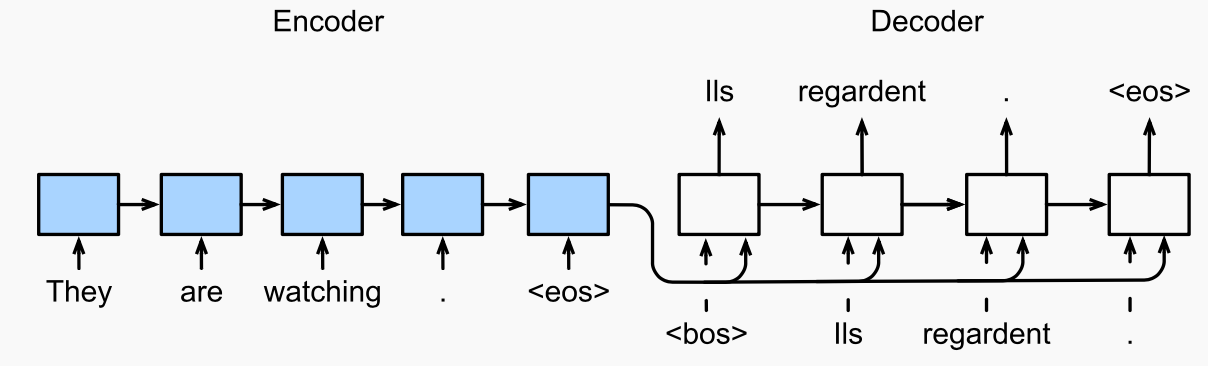
\includegraphics[height=2.5cm]{figures/rnn-enc-dec}
        \caption{10.7.1 from \href{https://d2l.ai/chapter_recurrent-modern/seq2seq.html}{d2l.ai}}
    \end{figure}
    \vspace{-1em}

    \begin{itemize}
        \item The \textbf{encoder} embeds the input recurrently
            and produce a \blue{context vector}
            $$
            h_t = \mathrm{RNNEncoder}(x_t, h_{t-1}), \quad
            \blue{c} = f(h_1,\ldots,h_n)
            $$
        \pause
    \item The \textbf{decoder}  produce the \green{output states} {recurrently}
            and map them to distributions over the output vocabulary
            $$\green{s_t} = \mathrm{RNNDecoder}(\pb{y_{t-1};c}, \green{s_{t-1}}), \quad
            p(y_t\mid y_{<t}, x) = \mathrm{softmax}(\mathrm{Linear}(\green{s_t}))
            $$
    \end{itemize}
\end{frame}

\begin{frame}
    {Bi-directional RNN encoder}
    The $\text{[Forbes]}_{??}$ building is at 60 Fifth Ave.
    \pause

    We may want the hidden state to summarize both \blue{left and right context}
    \pause

    \medskip
    \begin{columns}
        \begin{column}{0.5\textwidth}
    \begin{figure}
        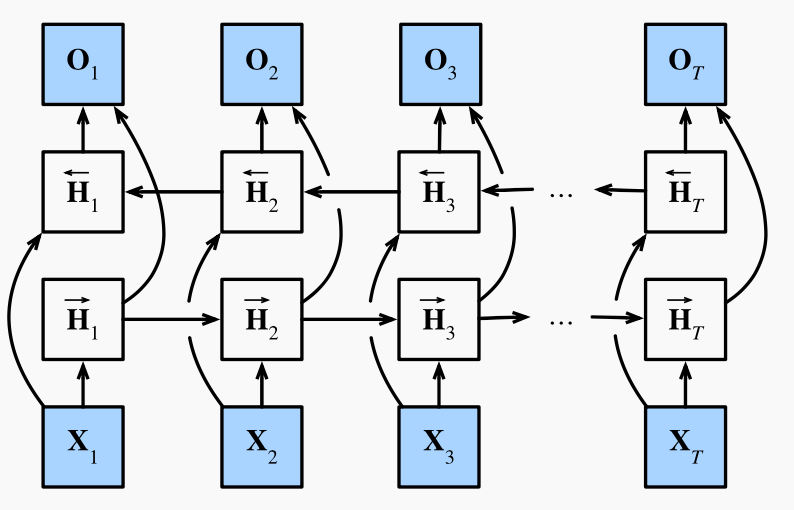
\includegraphics[height=3.5cm]{figures/birnn}
        \caption{10.4.1 from \href{https://d2l.ai/chapter_recurrent-modern/bi-rnn.html}{d2l.ai}}
    \end{figure}
        \end{column}
        \begin{column}{0.5\textwidth}
            \begin{wideitemize}
                \item Use two RNNs, one encode from left to right, the other from right to left
                \item Concatenate hidden states from the two RNNs
            \begin{align*}
                h_t &= [\overleftarrow{h_t}; \overrightarrow{h_t}]\\
                o_t &= Wh_t + b
            \end{align*}
            \end{wideitemize}
        \end{column}
    \end{columns}
\end{frame}

\begin{frame}
    {Multilayer RNN}
    \begin{columns}
        \begin{column}{0.5\textwidth}
    \begin{figure}
        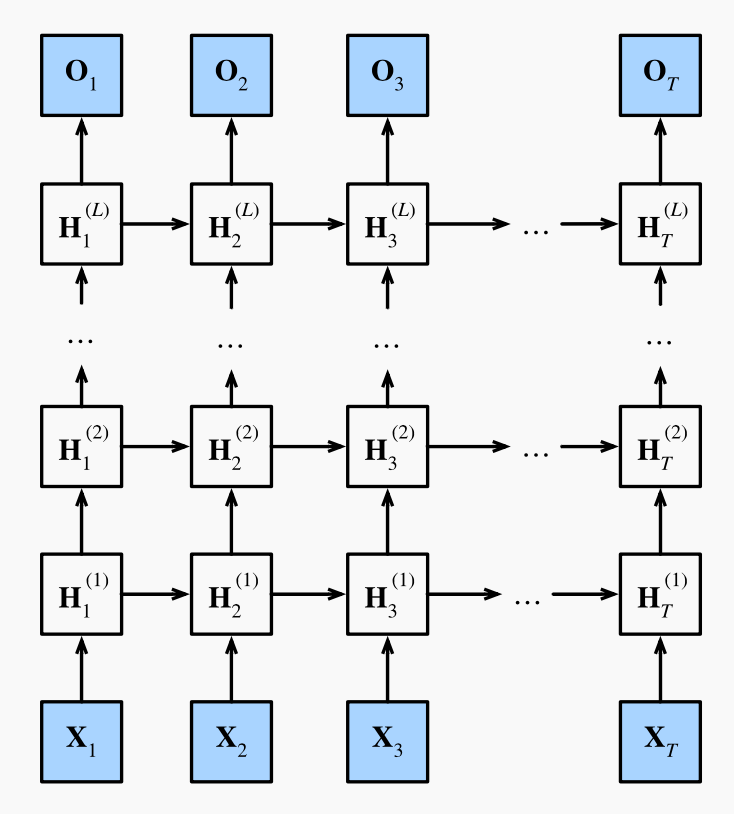
\includegraphics[height=4.5cm]{figures/multi-rnn}
        \caption{\href{https://d2l.ai/chapter_recurrent-modern/deep-rnn.html}{10.3.1} from {d2l.ai}}
    \end{figure}
        \end{column}
        \begin{column}{0.5\textwidth}
            \begin{wideitemize}
                \item Increase model capacity (scaling up) 
                \item Inputs to layer 1 are words
                \item Inputs to layer $j$ are outputs from layer $j-1$
                \item Typically 2--4 layers
            \end{wideitemize}
        \end{column}
    \end{columns}
\end{frame}

\begin{frame}
    {Encoder-decoder attention: motivation}

    Recall that the \blue{context vector} summarizes the input:
    $$
    {s_t} = \mathrm{RNNDecoder}(\pb{y_{t-1};\blue{c}}, {s_{t-1}})
    $$

    Should we use the same context vector for every decoding step?

    \pause
    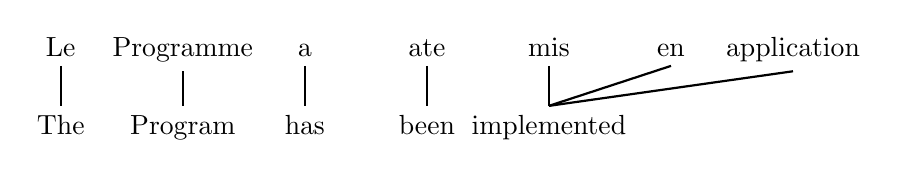
\begin{tikzpicture}
        \foreach \i/\w in {1/Le, 2/Programme, 3/a, 4/ate, 5/mis, 6/en, 7/application}{
            \node[anchor=base] (x\i) at(1.55*\i,0) {\w};
        }
        \foreach \i/\w in {1/The, 2/Program, 3/has, 4/been, 5/implemented}{
            \node[anchor=base] (y\i) at(1.55*\i,-1) {\w};
        }
        \path[draw, thick] (x1.south) -- (y1.north);
        \path[draw, thick] (x2.south) -- (y2.north);
        \path[draw, thick] (x3.south) -- (y3.north);
        \path[draw, thick] (x4.south) -- (y4.north);
        \path[draw, thick] (x5.south) -- (y5.north);
        \path[draw, thick] (x6.south) -- (y5.north);
        \path[draw, thick] (x7.south) -- (y5.north);
    \end{tikzpicture}

    We may want to ``look at'' different parts of the input during decoding.

\end{frame}

\begin{frame}
    {Encoder-decoder attention: motivation}

    Gradient vanishing for long distance dependence

    \begin{figure}
        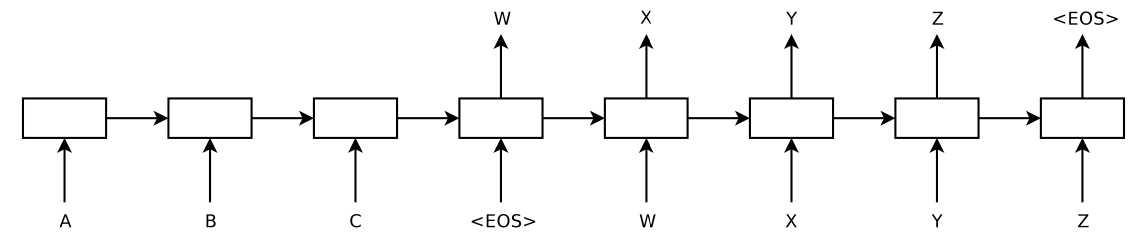
\includegraphics[height=2.5cm]{figures/s2s-ilya}
        \caption{From \href{https://arxiv.org/abs/1409.3215}{Sequence to Sequence Learning with Neural Networks} [Sutskever et al., 2014]}
    \end{figure}

    \pause
    We may want gradient to flow more directly from input to output
\end{frame}

\begin{frame}
    {Encoder-decoder attention: formalization}

    Recall that attention models interactions between two sets of objects:

    Which \blue{input tokens} are most relevant for generating the \red{next output} token? 

    \pause\medskip
    \begin{columns}
        \begin{column}{0.6\textwidth}
    \begin{wideitemize}[<+->]
        \item Query: decoder states $s_{t-1}$
        \item Key: encoder states $h_1,\ldots,h_n$
        \item Value: encoder states $h_1,\ldots,h_n$
        \item Attention context: $c_t = \sum_{i=1}^n \alpha(\red{s_{t-1}}, \blue{h_i}) h_i$
        \item Next state: $s_t = \mathrm{RNNDecoder}(\pb{y_{t-1};\green{c_t}}, s_{t-1})$
            \begin{itemize}
                \item \green{Dynamic} context vector instead of a fixed one
            \end{itemize}
    \end{wideitemize}
        \end{column}
        \begin{column}{0.4\textwidth}
            \onslide<+->{
            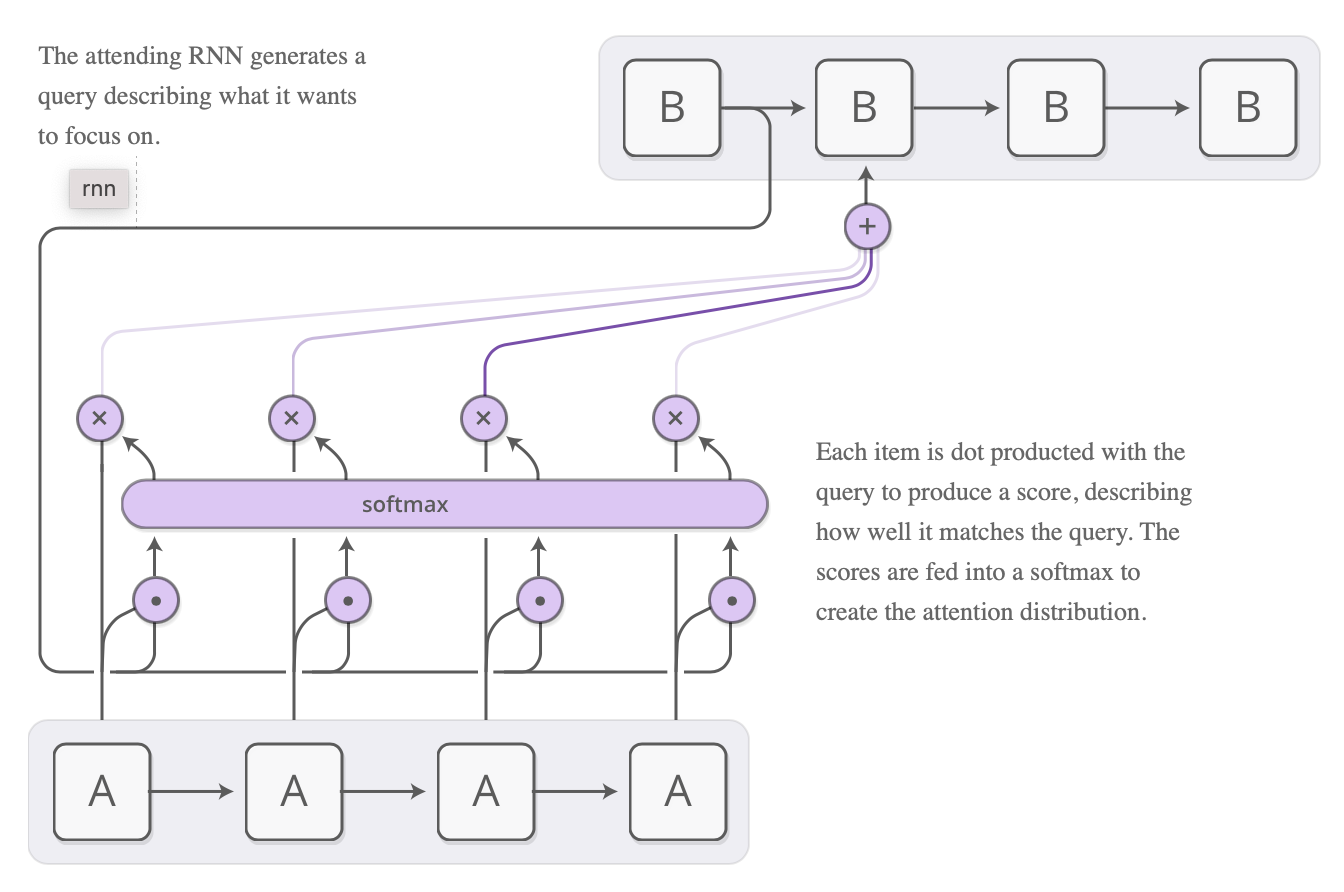
\includegraphics[height=4cm]{figures/s2s-attention}
            }
        \end{column}
    \end{columns}
\end{frame}

\begin{frame}
    {Summary so far}
    The outputs of an encoder can be used by (linear) classifiers for classification, sequence labeling, etc.

    A decoder is used to \blue{generate} a sequence of symbols.

    RNN encoder decoder model:\\
    \begin{itemize}
        \item Basic unit is an \blue{RNN} (or its variants like LSTM)
        \item Make it more expressive: \blue{bi-directional}, \blue{multilayer} RNN
        \item \blue{Encoder-decoder attention} helps the model learn input-output dependencies more easily
        \item Bi-directional LSTM is the go-to architecture for NLP tasks until around 2017
    \end{itemize}
\end{frame}

\begin{frame}
    {Transformer encoder decoder model}
    \begin{figure}
        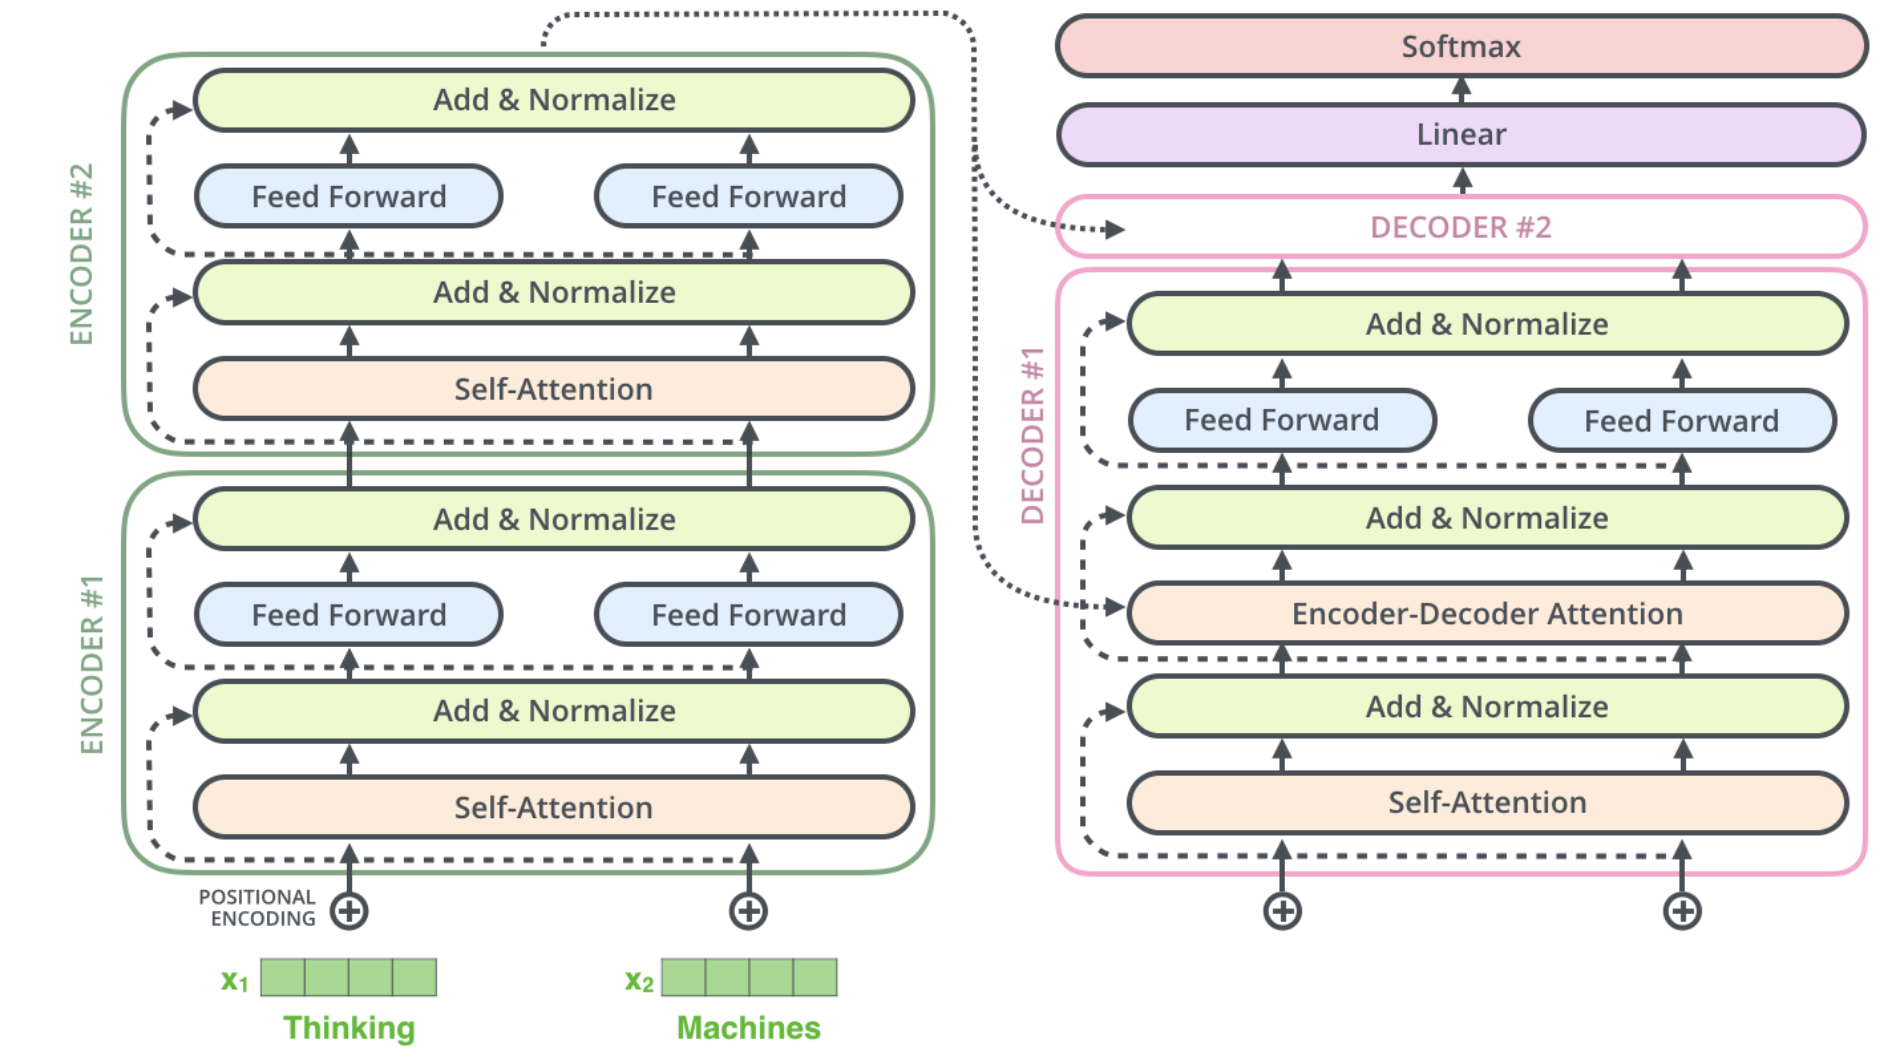
\includegraphics[height=5cm]{figures/transformer-enc-dec}
        \caption{From \href{https://jalammar.github.io/illustrated-transformer/}{illustrated transformer}}
    \end{figure}
    \vspace{-2em}

    \begin{itemize}
        \item Stack the tranformer block (typically 12--24 layers)
        \item Decoder has an additional encoder-decoder multi-head attention layer
    \end{itemize}
    %\pause\vspace{-1ex}
    %\think{Which part of the computation can be parallelized?}
\end{frame}

\begin{frame}
    {Encoder-decoder attention in Transformer}

    \begin{figure}
        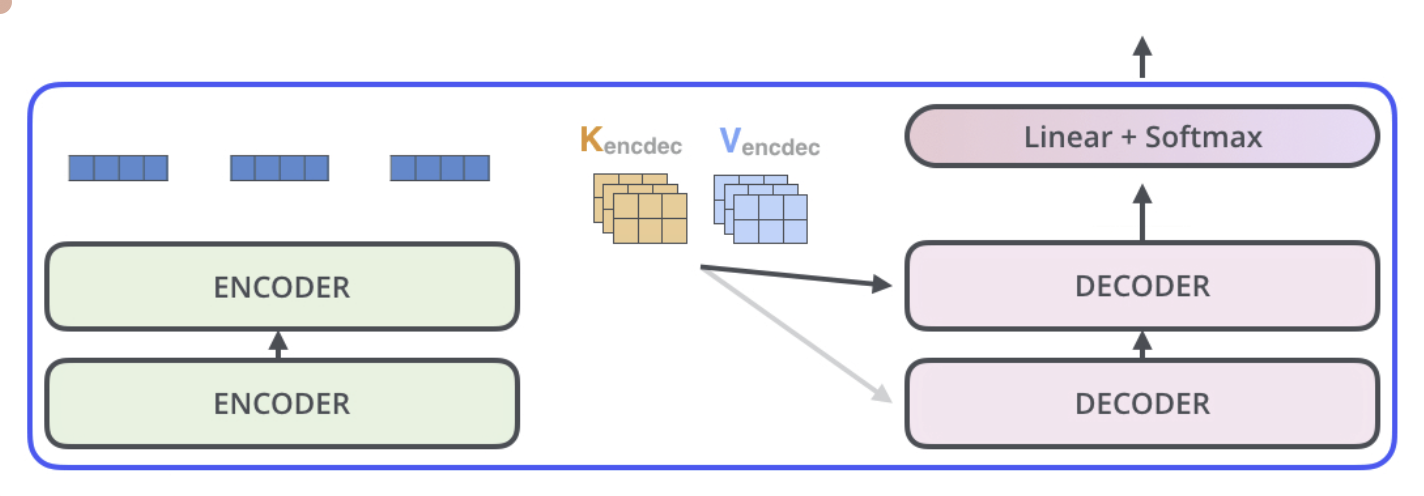
\includegraphics[height=3cm]{figures/encdec-attn}
        \caption{From \href{https://jalammar.github.io/illustrated-transformer/}{illustrated transformer}}
    \end{figure}

    \vspace{-1cm}
    \begin{align}
        \mathrm{TransformerEncoder}(x_1,\ldots,x_n) &= [h_1,\ldots,h_n] = H_{\text{enc}}\\
        K_{\text{encdec}} &= H_{\text{enc}} W^K \\
        V_{\text{encdec}} &= H_{\text{enc}} W^V \\\pause
        \mathrm{DecoderSelfAttention}(y_1,\ldots,y_t) &= [s_1,\ldots,s_t]\\
        q_t &= s_t W^Q
    \end{align}
\end{frame}

\begin{frame}
    {Impact on NLP}
    \begin{itemize}
        \itemsep1em
        \item Initially designed for sequential data and obtained SOTA results on MT
        \item Replaced recurrent models (e.g. LSTM) on many tasks
        \item Enabled large-scale training which led to pre-trained models such as BERT and GPT-2
    \end{itemize}

    Why are they so powerful?
\end{frame}

\begin{frame}
    {Autoregressive generative models}

    Generating sequences one token at a time from left to right

    \begin{enumerate}
        \item \green{Le Programme    a    ate    mis    en application}
            $\to$ \red{The}
        \item \green{Le Programme    a    ate    mis    en application},
            \blue{The}
            $\to$ \red{program}
        \item \green{Le Programme    a    ate    mis    en application},
            \blue{The program}
            $\to$ \red{has}
        \item \green{Le Programme    a    ate    mis    en application},
            \blue{The program has}
            $\to$ \red{been}
        \item ...
    \end{enumerate}

\end{frame}

\begin{frame}
    {Autoregressive generative models}

    Generating sequences one token at a time from left to right

    $$
    \mathrm{Encoder}(\green{x_1,\ldots,x_n}) = [h_1,\ldots,h_n]
    $$

    \begin{enumerate}
        \item $\mathrm{Decoder}([h_1,\ldots,h_n]) \to \red{y_1}$
        \item $\mathrm{Decoder}([h_1,\ldots,h_n], \blue{y_1}) \to \red{y_2}$
        \item $\mathrm{Decoder}([h_1,\ldots,h_n], \blue{y_1,y_2}) \to \red{y_3}$
        \item $\mathrm{Decoder}([h_1,\ldots,h_n], \blue{y_1,y_2,y_3}) \to \red{y_4}$
        \item ...
    \end{enumerate}
\end{frame}

\begin{frame}
    {Autoregressive generative models}

    Is this the only way of modeling and generating text?\pause

    We want to learn $p(y\mid x)$ \\
    \begin{itemize}
        \item Decompose the probability using \textbf{chain rule of probability} 
            \begin{align*}
                p(y\mid x) &= p(y_1\mid x)p(y_2\mid y_1, x)\ldots p(y_m\mid y_{m-1},\ldots,y_1, x) \\
                &= \prod_{i=1}^m p(y_i\mid y_{<i}, x)
            \end{align*}
        \item But we don't have to decompose it from left to right
    \end{itemize}
\end{frame}

\begin{frame}
    {Training}

    We are given a dataset $\sD = \pc{(x^{(i)},y^{(i)})}_{i=1}^N$ of input and output sequences

    Maximum likelihood estimation:\\
    $$
    \max \sum_{(x,y)\in\sD} \sum_{j=1}^m \log p(y_j\mid y_{<j}, x; \theta)
    $$
    \pause

    What is the prefix $y_{<j}$?\\[1ex]\pause
    %\only<+>{
    %    Option 1: whatever generated by the model 
    %\begin{figure}
    %    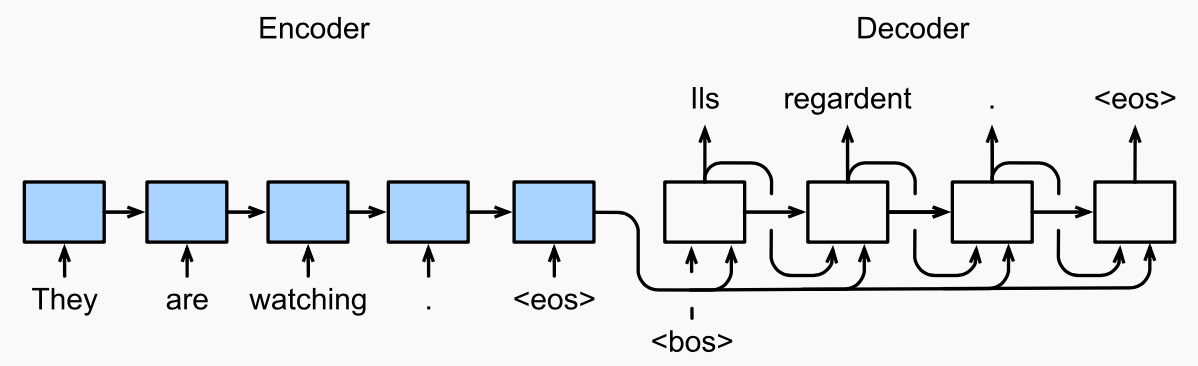
\includegraphics[height=2.5cm]{figures/rnn-enc-dec-gen}
    %    \caption{10.7.1 from \href{https://d2l.ai/chapter_recurrent-modern/seq2seq.html}{d2l.ai}}
    %\end{figure}
    %    }
            \onslide<+->{
        Use the groundtruth prefix (\textbf{teacher forcing})
    %\begin{figure}
    %    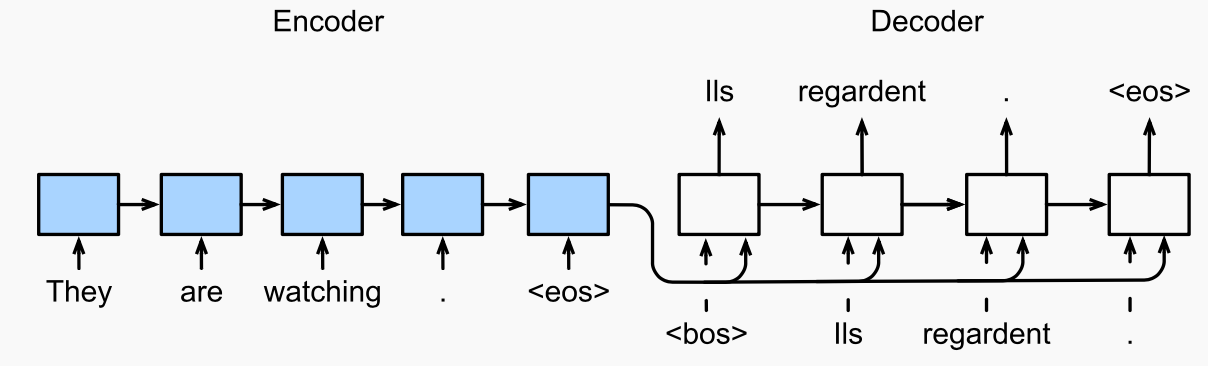
\includegraphics[height=2.5cm]{figures/rnn-enc-dec}
    %    \caption{10.7.3 from \href{https://d2l.ai/chapter_recurrent-modern/seq2seq.html}{d2l.ai}}
    %\end{figure}
        }
\end{frame}

\begin{frame}
    {Start and end symbols}
    Which one is more likely?

    \begin{align*}
    p(\text{The} \mid \text{Le Programme    a    ate    mis    en application}) \\
    p(\text{The program has been implemented} \mid \text{Le Programme    a    ate    mis    en application}) \\
    \end{align*}

    \pause
    Use sequence start and end symbols to model sequence length
    \begin{itemize}
        \item {Le Programme    a    ate    mis    en application}
            $\to$ \red{<s>} The ... \red{</s>}
    \end{itemize}
\end{frame}


\begin{frame}
    {Decoder attention masking}

    Recall that the output of self-attention depends on all tokens $y_1,\ldots y_m$.

    But the decoder is supposed to model $p(y_t\mid y_{<t}, x)$.

    It should not look at the ``future'' ($y_{t+1},\ldots,y_m$)!

    \pause
    How do we fix the decoder self-attention?\\
    \begin{wideitemize}
        \item Mathematically, changing the input values and keys suffices.
        \item Practically, set $a(s_i, s_j)$ to $-\inf$ for all $j>i$ and for $i=1,\ldots,m$.
            \begin{itemize}
                \item The attention matrix is a lower-triangular matrix.
            \end{itemize}
    \end{wideitemize}
\end{frame}


\begin{frame}
    {Inference}
    %How do we generate sequences given a trained model?
    %\begin{figure}
    %    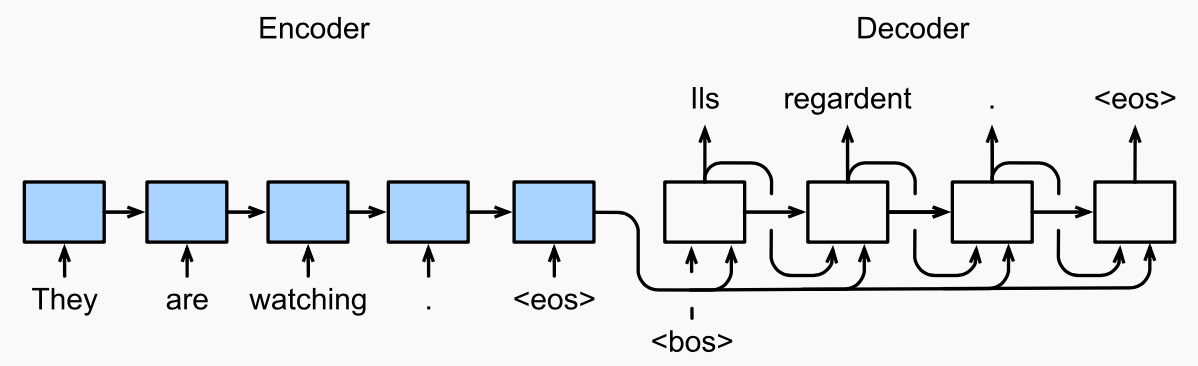
\includegraphics[height=2.5cm]{figures/rnn-enc-dec-gen}
    %    \caption{10.7.1 from \href{https://d2l.ai/chapter_recurrent-modern/seq2seq.html}{d2l.ai}}
    %\end{figure}

    Suppose we have a trained model $p(y\mid x;\theta)$.

    The model defines \blue{a probability distribution} over all possible sequences.

    But we want to output a single \blue{sequence}.

    The \textbf{decoding} problem: How do we predict a sequence from the model?
\end{frame}

\begin{frame}
    {Inference}

    \textbf{Argmax decoding}: 
    $$
    \hat{y} = \argmax_{y\in\red{\sV_{\text{out}}^n}} p(y\mid x; \theta)
    $$
    \vspace{-1em}
    \begin{itemize}
        \item Return the \red{most likely sequence}
        \item But exact search is intractable 
    \end{itemize}

    \pause
    Approximate search:\\
    \begin{itemize}
        \item \textbf{Greedy decoding}: return the \green{most likely symbol} at each step
            $$
            y_t = \argmax_{y\in\green{\sV_{\text{out}}}} p(y\mid x, \hat{y}_{<t}; \theta)
            $$
    \end{itemize}

    When to stop?
\end{frame}

\begin{frame}
    {Approximate decoding: beam search}

    \textbf{Beam search}: maintain $k$ (beam size) highest-scored \blue{partial} solutions at every step 

    $$
    \mathrm{score}(\blue{y_1,\ldots,y_t}) = \sum_{i=1}^t \log p_\theta(y_i\mid y_{<i})
    $$
    
    %Example: $|\sV|=5, k=2$
    %\vspace{-1em}
    %\begin{figure}
    %    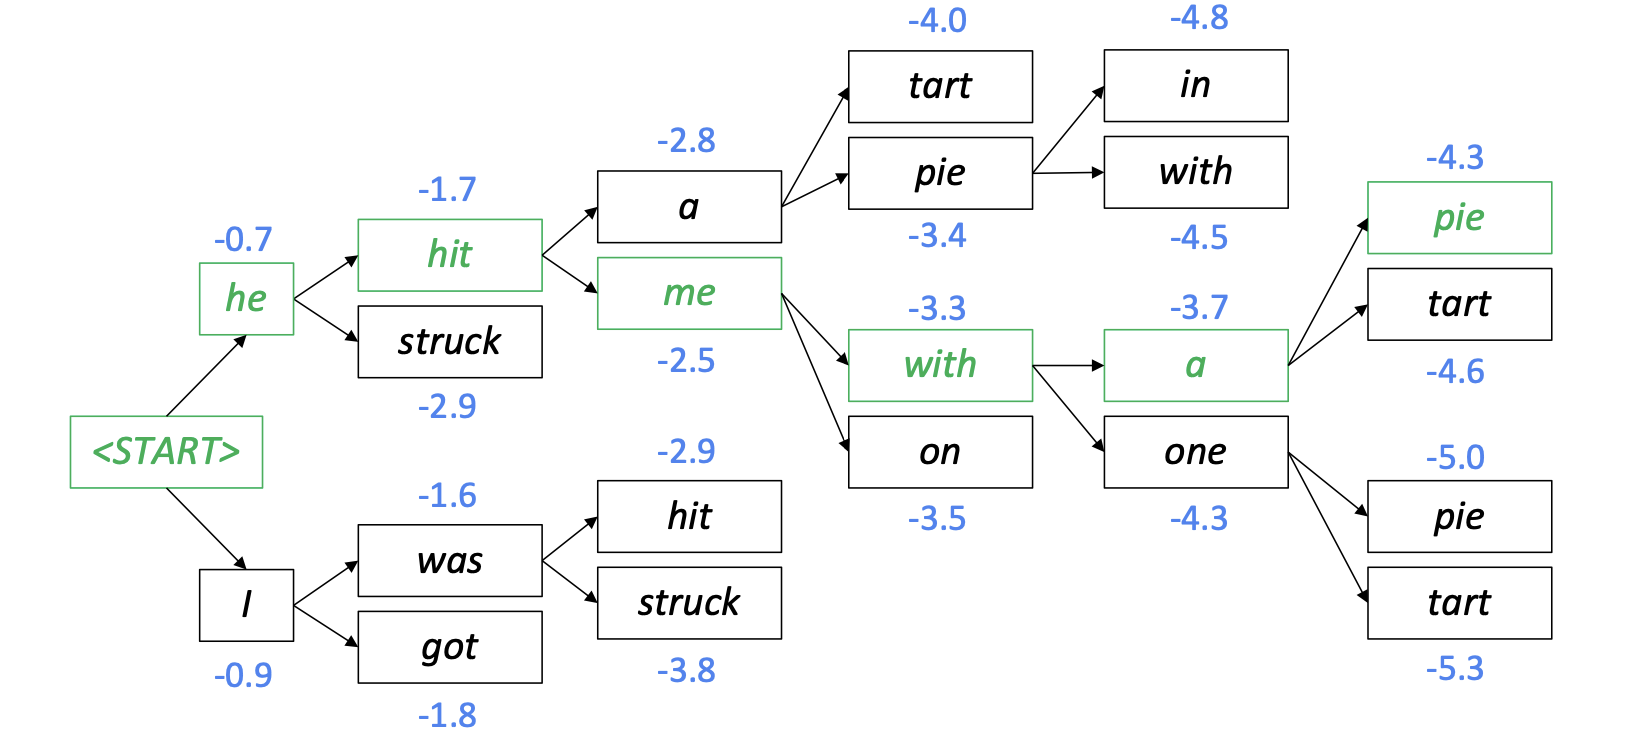
\includegraphics[height=4cm]{figures/beam-search}
    %\end{figure}
    %\vspace{-1em}
    \pdfnote{
        At each step, we want to find the partial sequence with the highest score.
        At the end, we would have the highest scoring complete sequence.
        But isn't this more expensive?
        We need to use DP here by reusing previous result.
        By chain rule, at each step, we can reuse previous compute.
        But still, this isn't saving us much compute, because we are still enumerating the score of all sequences.
        The main trick in beam search is to reduce the search space at each step to a constant number, i.e. the beam size.
        Basically, we only save the top-k partial sequences at each step.
    }

    \begin{wideitemize}
        \item At each step, we have a set of $k$ partial hypotheses (prefixes)
        \item Use the autoregressive model, we can expand all hypotheses by one more token (how many hypotheses do we have now?)
        \item Evaluate the score of all hypotheses and keep the top $k$
    \end{wideitemize}
\end{frame}

\begin{frame}
    {Beam search example}
    \begin{figure}
        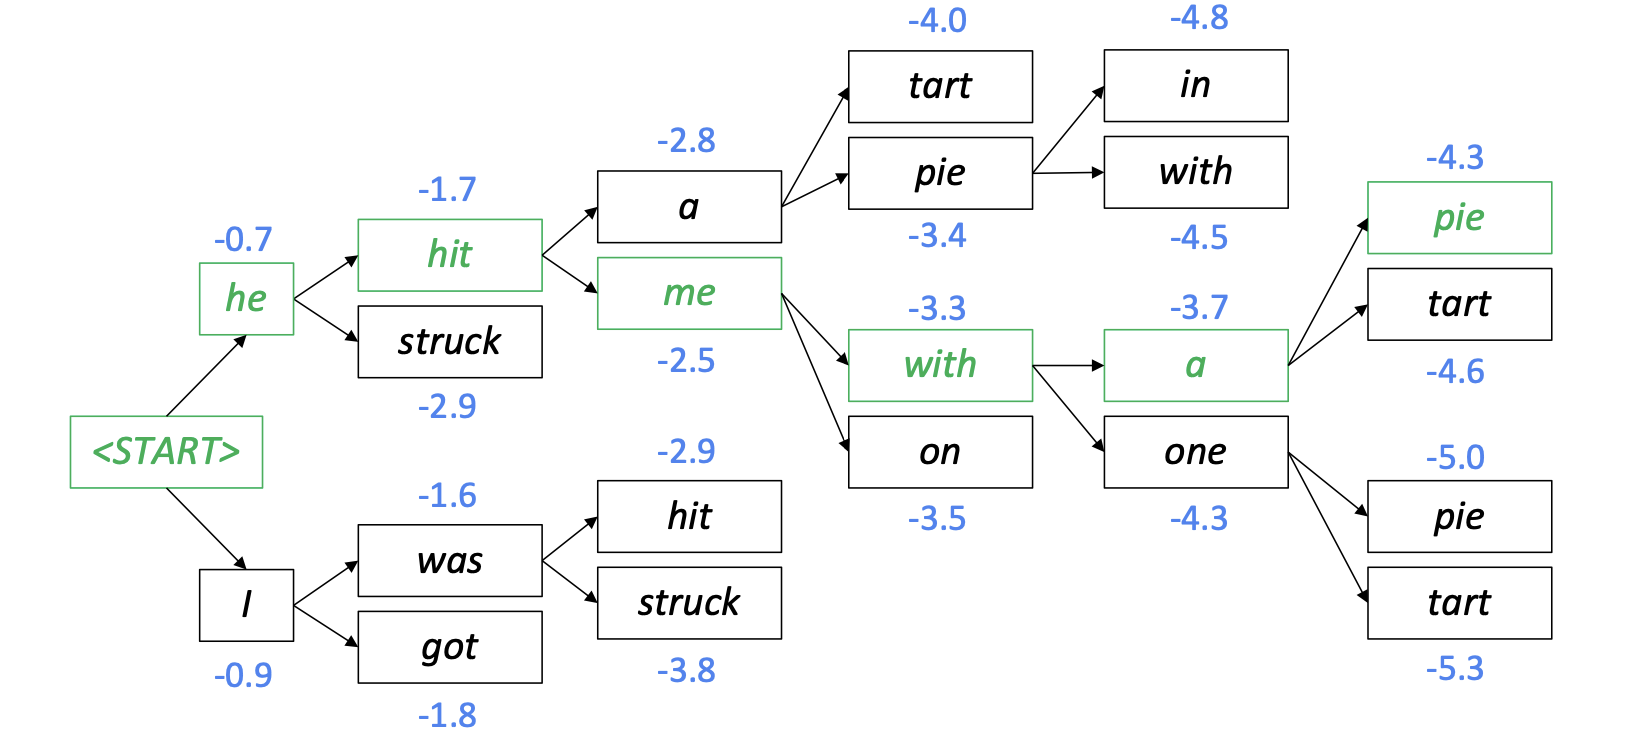
\includegraphics[height=5cm]{figures/beam-search}
        \caption{Figure from Chris Manning}
    \end{figure}

    \pause
    Stop when all hypotheses in the beam has terminated or when hitting a limit of number of steps.
    % beam size = 1 or hard limit of steps
\end{frame}

\begin{frame}
    {Is argmax the right decoding objective?}
    \blue{High likelihood} can be correlated with \red{low quality} outputs! \href{https://arxiv.org/abs/2004.10450}{[Zhang et al., 2020]}
    \begin{figure}
        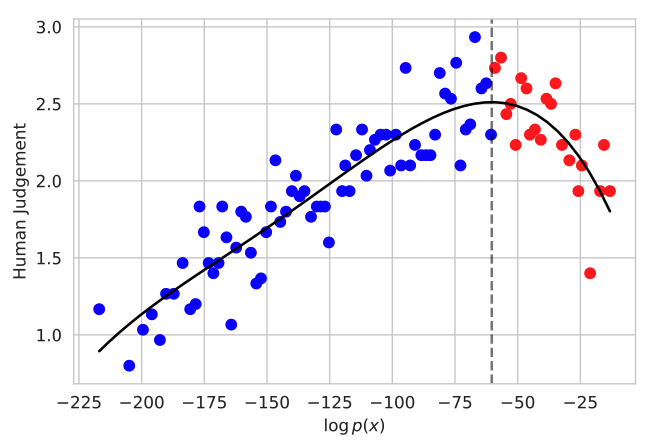
\includegraphics[height=3cm]{figures/likelihood-trap}\\
        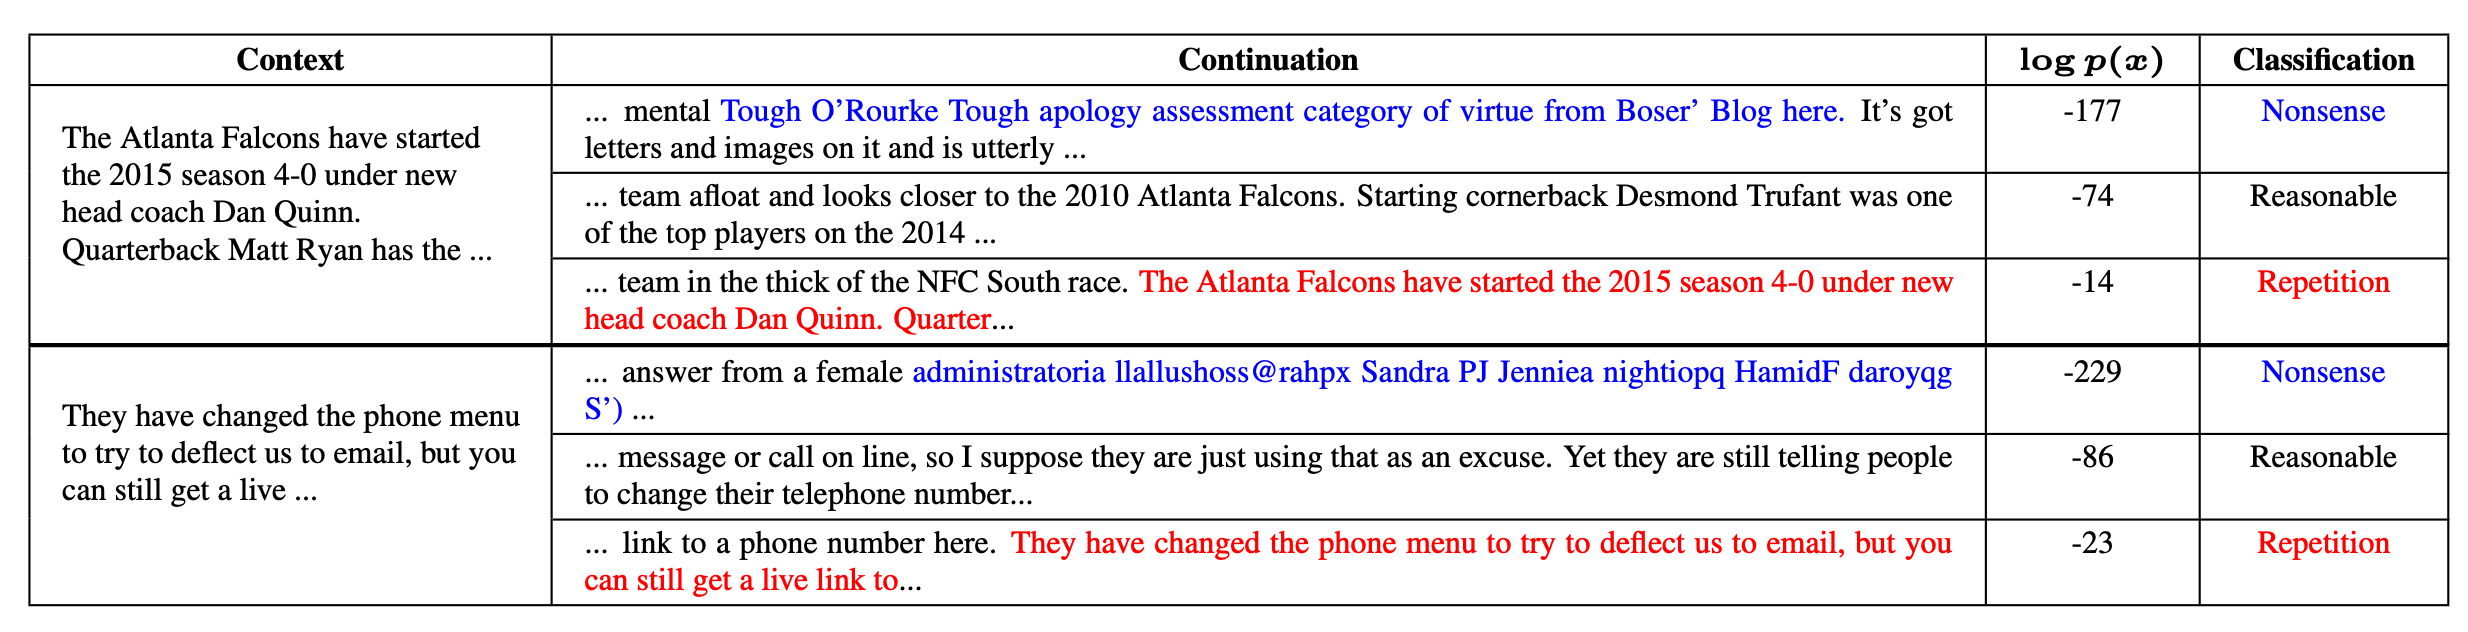
\includegraphics[width=\textwidth]{figures/likelihood-trap-ex}
    \end{figure}
\end{frame}

\begin{frame}
    {Is argmax the right decoding objective?}

    In practice, argmax decoding has been observed to lead to\\
    \begin{itemize}
        \item \red{Repetitive generations}, e.g., 
            {\small
                ``..., was conducted by researchers from the Universidad Nacional Autonoma de Mexico (UNAM) and {the Universidad Nacional Autonoma de Mexico (UNAM/Universidad Nacional Autonoma de Mexico/Universidad Nacional Autonoma de Mexico/Universidad Nacional Autonoma...}''}
            \item \red{Empty or extremely short translations} with large beam size in MT
    \end{itemize}

    \pause
    {\bf Hypotheses}:\\
    \begin{itemize}
        \item Models don't fit the data well \\
            {\em But problem doesn't go away with larger model and data}
        \item Distribution shift during inference (more on this later)\\
            {\em Need more evidence}
        \item Training data contains repetition
    \end{itemize}
\end{frame}

\begin{frame}
    {Sampling-based decoding}
    If we have learned a perfect $p(y\mid x)$, shouldn't we just sample from it?
    \pause

    \textbf{Sampling} is easy for autoregressive models:\\
    \begin{itemize}
        \item While output is not \texttt{EOS}
            \begin{itemize}
                \item \blue{Sample next word} from $p(\cdot\mid \text{prefix}, \text{input};\theta)$
                \item Append the word to prefix
            \end{itemize}
    \end{itemize}

    \pause
    Standard sampling often produces \red{non-sensical} sentences:\\
    \begin{itemize}
        \item[] {\footnotesize They were cattle called Bolivian Cavalleros; they live in a remote desert uninterrupted by town, and they speak huge, beautiful, paradisiacal Bolivian linguistic thing.}
    \end{itemize}

    \textbf{Idea}: \blue{modify the learned distrubtion} $p_\theta$ before sampling to avoid bad generations 
\end{frame}

\begin{frame}
    {Tempered sampling}

    \textbf{Intuition}: concentrate probability mass on highly likely sequences 

    \blue{Scale scores} (from the linear layer) before the softmax layer:\\
    \begin{align*}
        p(y_t=w \mid y_{<t},x) &\propto \exp\p{\mathrm{score}(w)}\\
        q(y_t=w \mid y_{<t}, x) &\propto \exp\p{\mathrm{score}(w)/{\color{blue}T}} 
        \quad \text{where } T\in(0, +\infty)
    \end{align*}
    \pause
    \vspace{-2em}
    \begin{itemize}
        \item What happends when $T\to 0$ and $T\to +\infty$?
        \item Does it change the rank of $y$ according to likelihood?
        \item Typically we chooose $T\in (0, 1)$, which makes the distribution \blue{more peaky}.
    \end{itemize}
\end{frame}

\begin{frame}
    {Truncated sampling}

    Another way to focus on highly likely sequences: \blue{truncate the tail} of the distribution

    \textbf{Top-k sampling}:\\
    \begin{itemize}
        \item Rank all tokens $w\in\sV$ by $p(y_t=w\mid y_{<t},x)$
        \item Only keep the top $k$ of those and renormalize the distribution
    \end{itemize}

    Effect of $k$:\\
    \begin{itemize}
        \item Large $k$: more \green{diverse} but possibly \red{degenerate} outputs
        \item Small $k$: more \red{generic} but \green{safe} outputs
    \end{itemize}
\end{frame}

\begin{frame}
    {Truncated sampling}
    Which $k$ to choose?
    \begin{figure}
        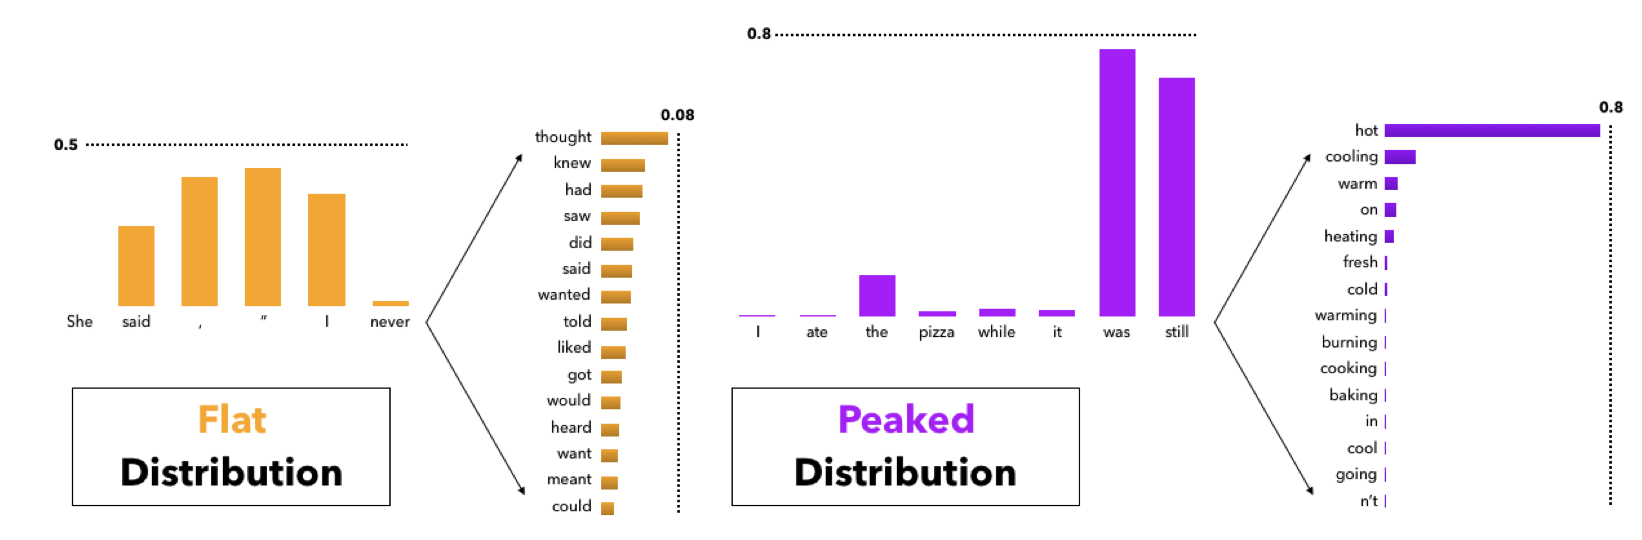
\includegraphics[width=0.9\textwidth]{figures/dynamic-k}
        \caption{From the \href{https://arxiv.org/pdf/1904.09751.pdf}{nucleus sampling} paper by Holtzman et al., 2020}
    \end{figure}
    Using a single $k$ on different next word distributions may be suboptimal
\end{frame}

\begin{frame}
    {Truncated sampling}
    
    \textbf{Top-p sampling}:\\
    \begin{itemize}
        \item Rank all tokens $w\in\sV$ by $p(y_t=w\mid y_{<t},x)$
        \item Keep only tokens in the top $p$ probability mass
            and renormalize the distribution
        \item The corresponding \blue{$k$ is dynamic}:
            \begin{itemize}
            \item Start with $k=1$, increment until the cumulative probability mass $>p$
            \end{itemize}
    \end{itemize}
    \begin{figure}
        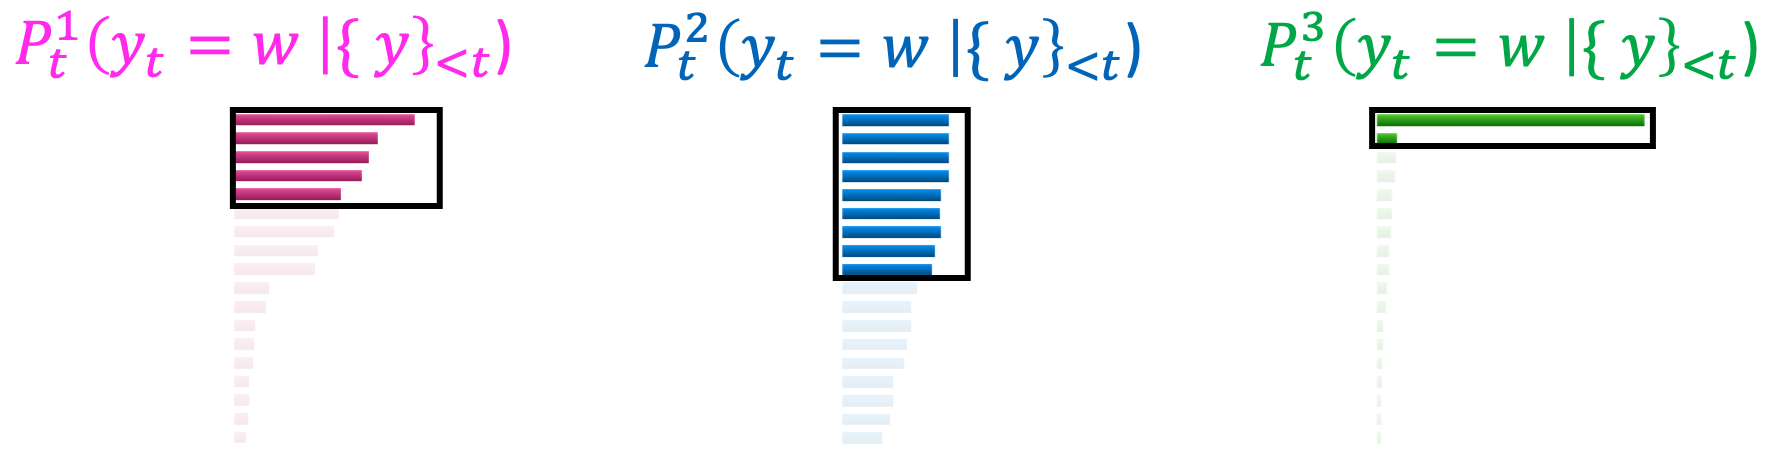
\includegraphics[width=0.8\textwidth]{figures/top-p}
        \caption{From Xiang Li's slides}
    \end{figure}
\end{frame}

\begin{frame}
    {Decoding in practice}
    \begin{itemize}
        \itemsep1em
        \item Can combine different tricks (e.g., temperature + beam search, temperature + top-$k$)
        \item Use beam search with small beam size for tasks where there exists a correct answer, e.g. machine translation
        \item Use top-$k$ or top-$p$ for open-ended generation, e.g. story generation, chit-chat dialogue
        \item As models getting better/larger, sampling-based methods tend to work better
    \end{itemize}
\end{frame}

\begin{frame}
    {Exposure bias}
    Problem with teacher forcing:\\
    \begin{itemize}
        \item During training, the model only sees \blue{groundtruth} prefix
        \item During inference, the model sees \red{generated} prefix, which may deviate from the training prefix distribution
        \item When this happends, the model behavior is underspecified.
    \end{itemize}

    \begin{figure}
        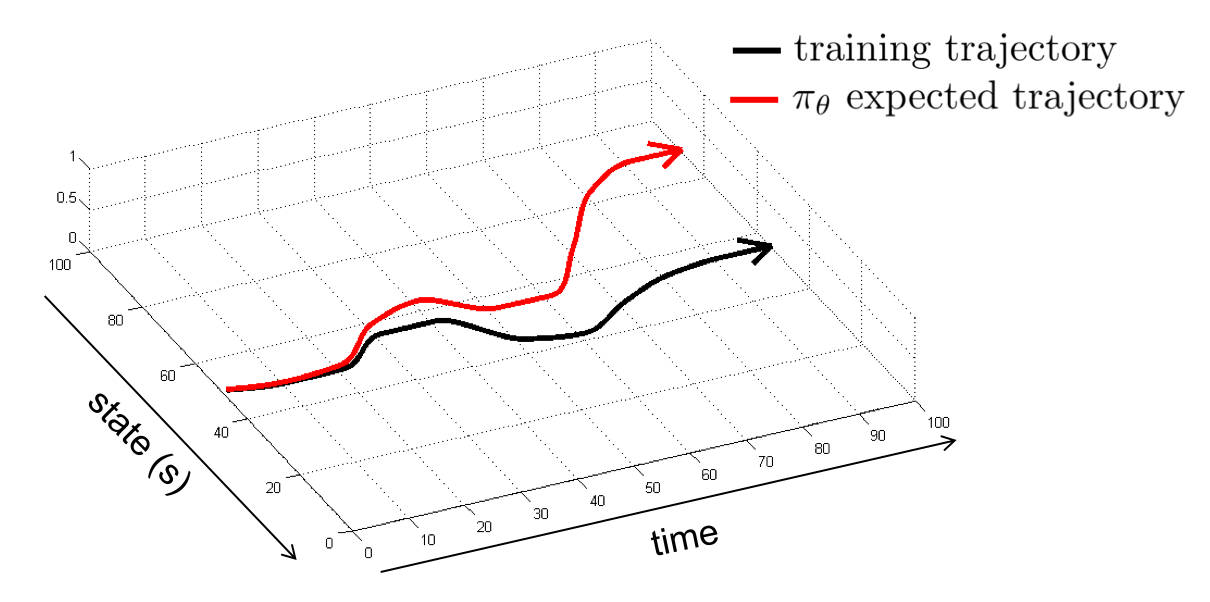
\includegraphics[height=0.5\textheight]{figures/exposure}
    \end{figure}
\end{frame}

\begin{frame}
    {Exposure bias}
    Solutions:\\
    \begin{itemize}
        \item \blue{Avoid deviating from the training prefix distribution}
            \begin{itemize}
                \item Better modeling: reduce errors at each step
                \item Better decoding: stay within the high likelihood region (later)
            \end{itemize}
        \pause
    \item \blue{Teaching the model how to behave on out-of-distribution prefix} %$\quad$ 
            \begin{itemize}
                \item Better learning: updating models based on the goodness of the {\em generated} sequence
                    \pause
                \item[] {\em\red{additional supervision required}}
                \item[] {\em\red{computationally more expensive}}
            \end{itemize}
    \end{itemize}
\end{frame}

\end{document}
